\chapter{项目设计}

\section{类图说明}



	我们的设计主要分为6个部分,分别是规则解析部分,规则实体/检查部分,报告部分,RUCM解析部分自然语言处理部分以及图形界面部分。接下来分别说明每个部分重要的具体类图设计。
		\begin{figure}
		\centering
		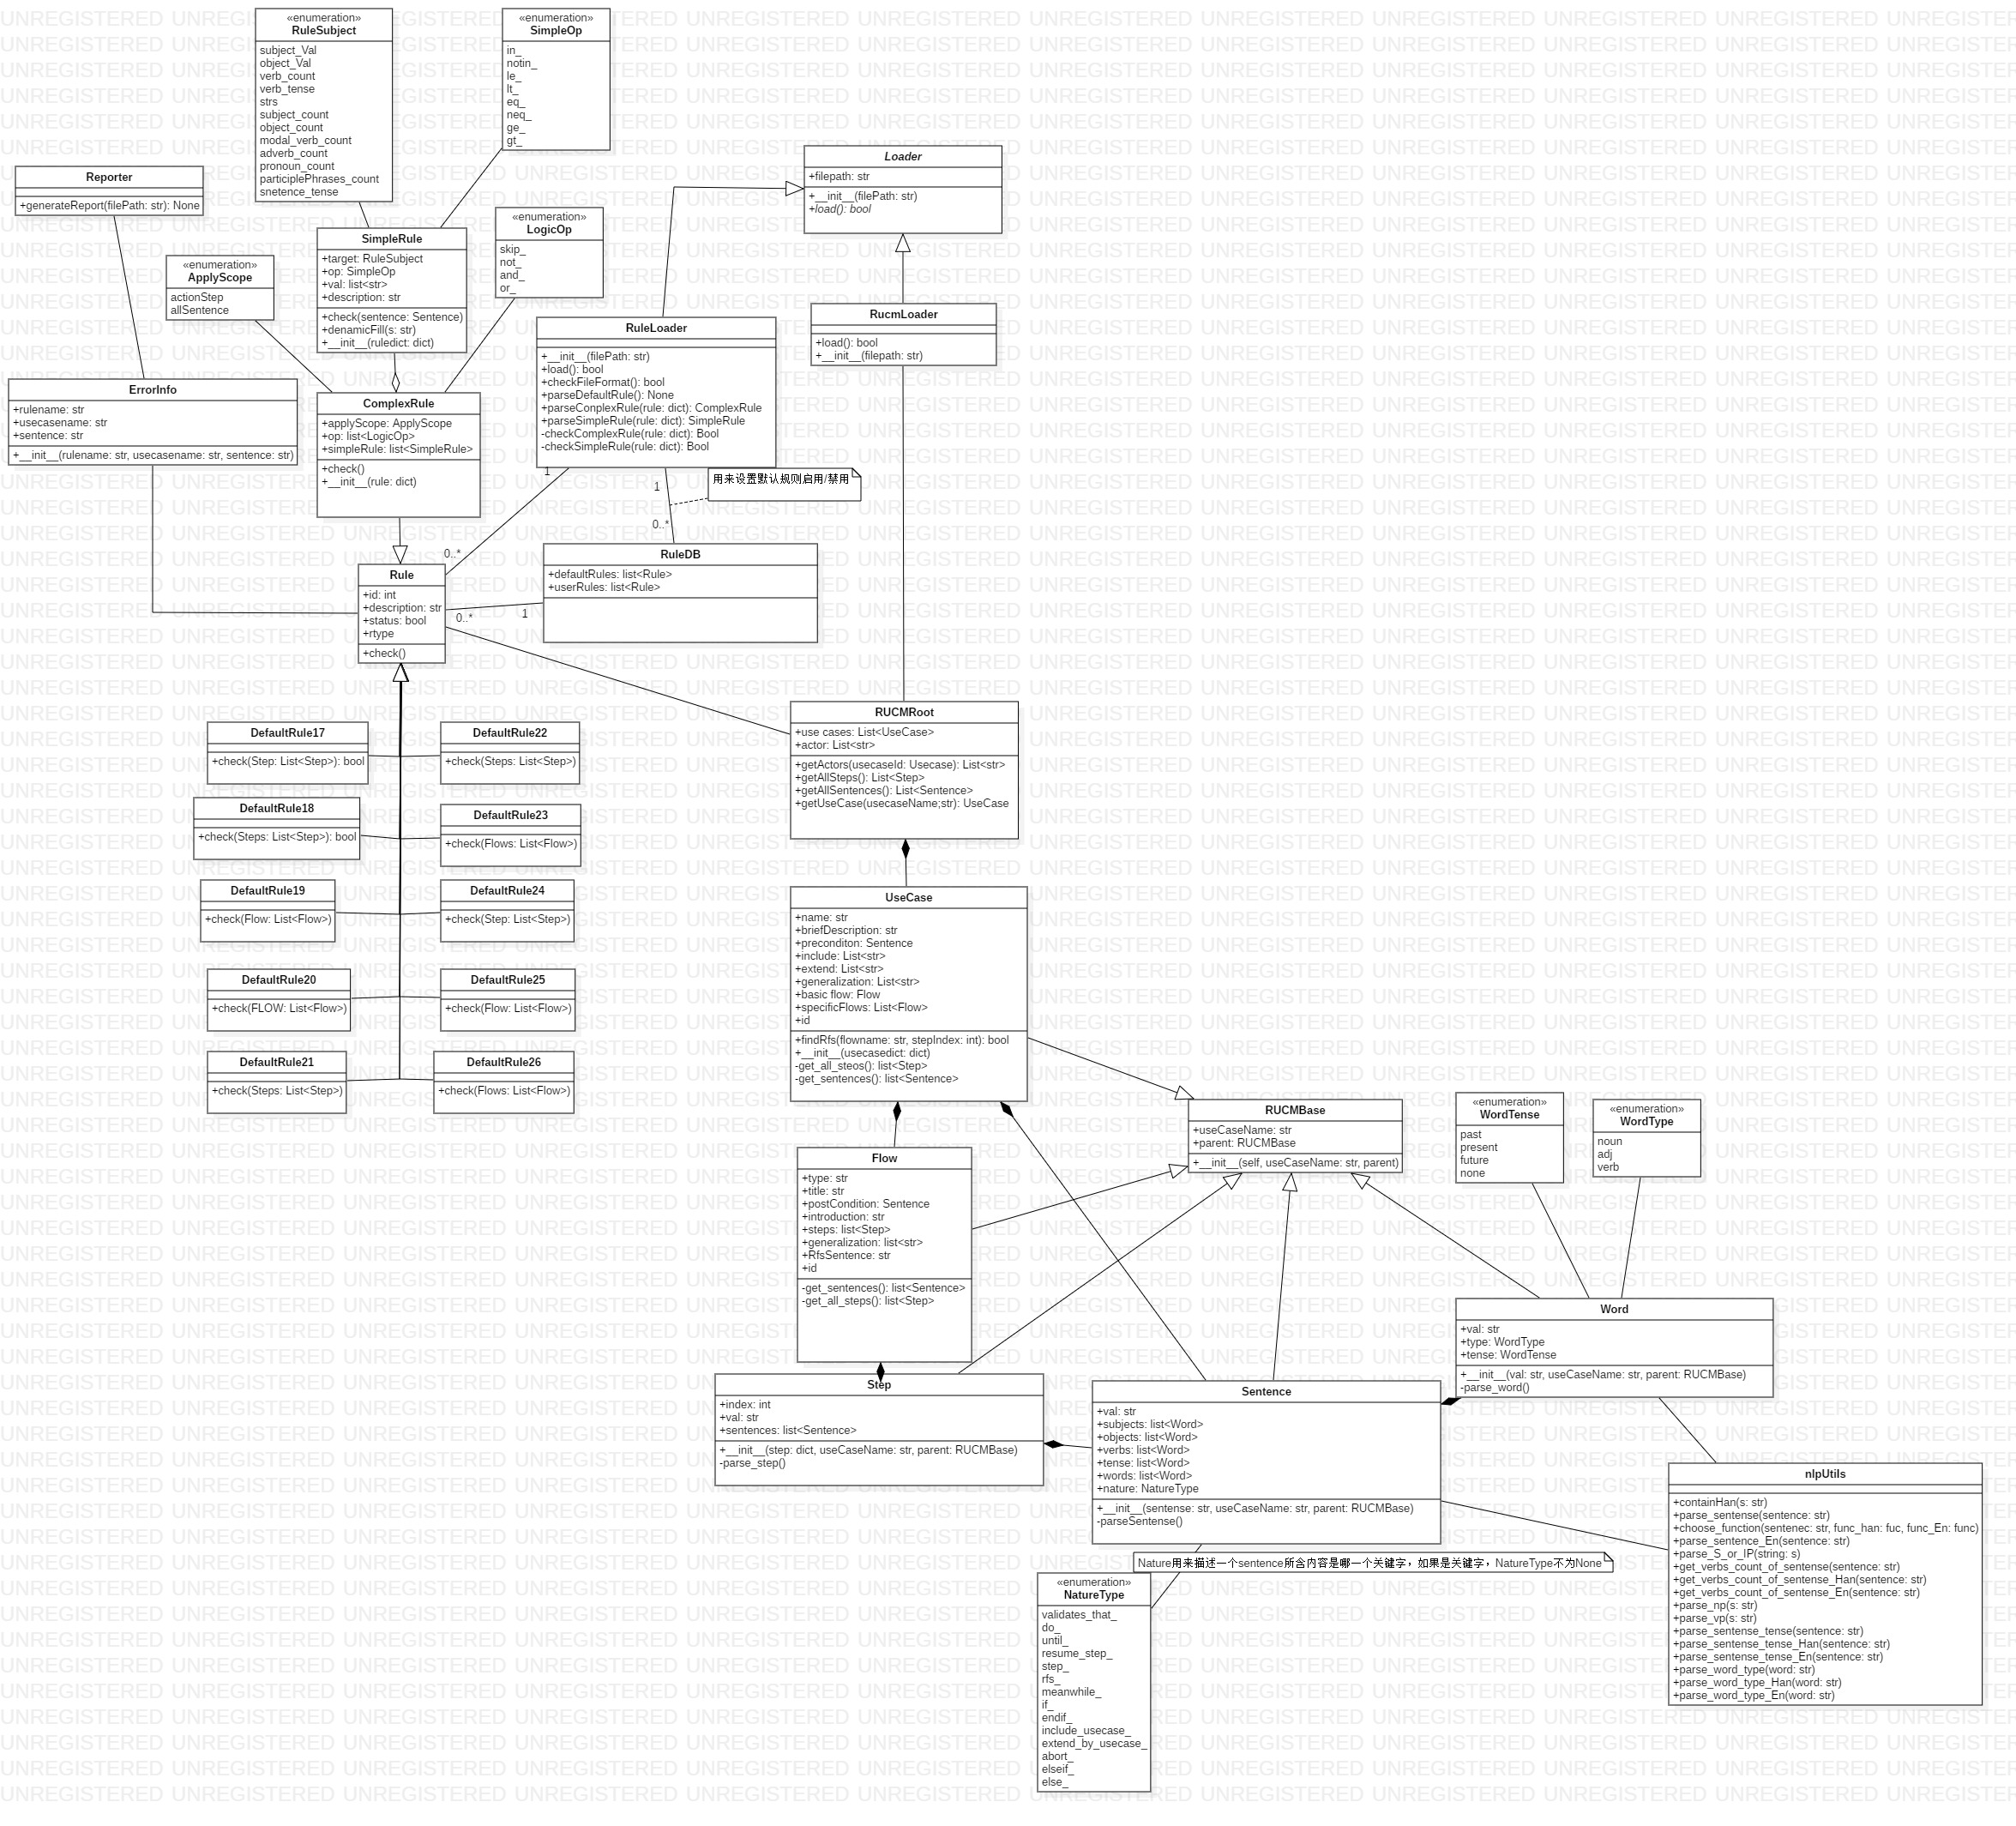
\includegraphics[width=1\textwidth]{./src/classDiagram_overview.jpg} 
		\caption{主体部分类图概览} 
		\label{key}
	\end{figure}

    \subsection{规则解析部分}
   		如图\ref{classDiagram_rule}所示,规则解析由类RuleLoader和RuleDB组成,RuleLoader的作用是将规则文件解析成ComplexRule/DefaultRule等类,装入ruleDB中。\\
    \begin{itemize}
    	

    	\item 	RuleLoader:\\
    	load()->bool:进行文件解析。文件解析结果将直接存放在RuleDB中。返回值代表是否解析成功\\
    	chekFileFormat(rule:dict)->bool:检查文件格式是否符合要求,包含检查相应的字段是否存在,字段的值是否合法,各个字段之间的关系是否符合约束\\
    	parseDefaultRule(rule:dict):解析默认规则\\
    	parseComplexRule(rule:dict):解析复合规则字典,具体规则格式详见rule-template.md\\
    	parseSimpleRule(rule:dict):解析简单规则\\
    	checkComplexRule(rule:dict):检查复合规则格式\\
    	checkSimpleRule(rule:dict):检查简单规则格式
    	\item 	RuleDB:\\
    	ruleDB为静态数据类,它根据两部分组成,分别是用户定义规则列表(userRules:list)和默认规则列表(userRules:list)组成\\
    	\begin{figure}
    		\centering
    		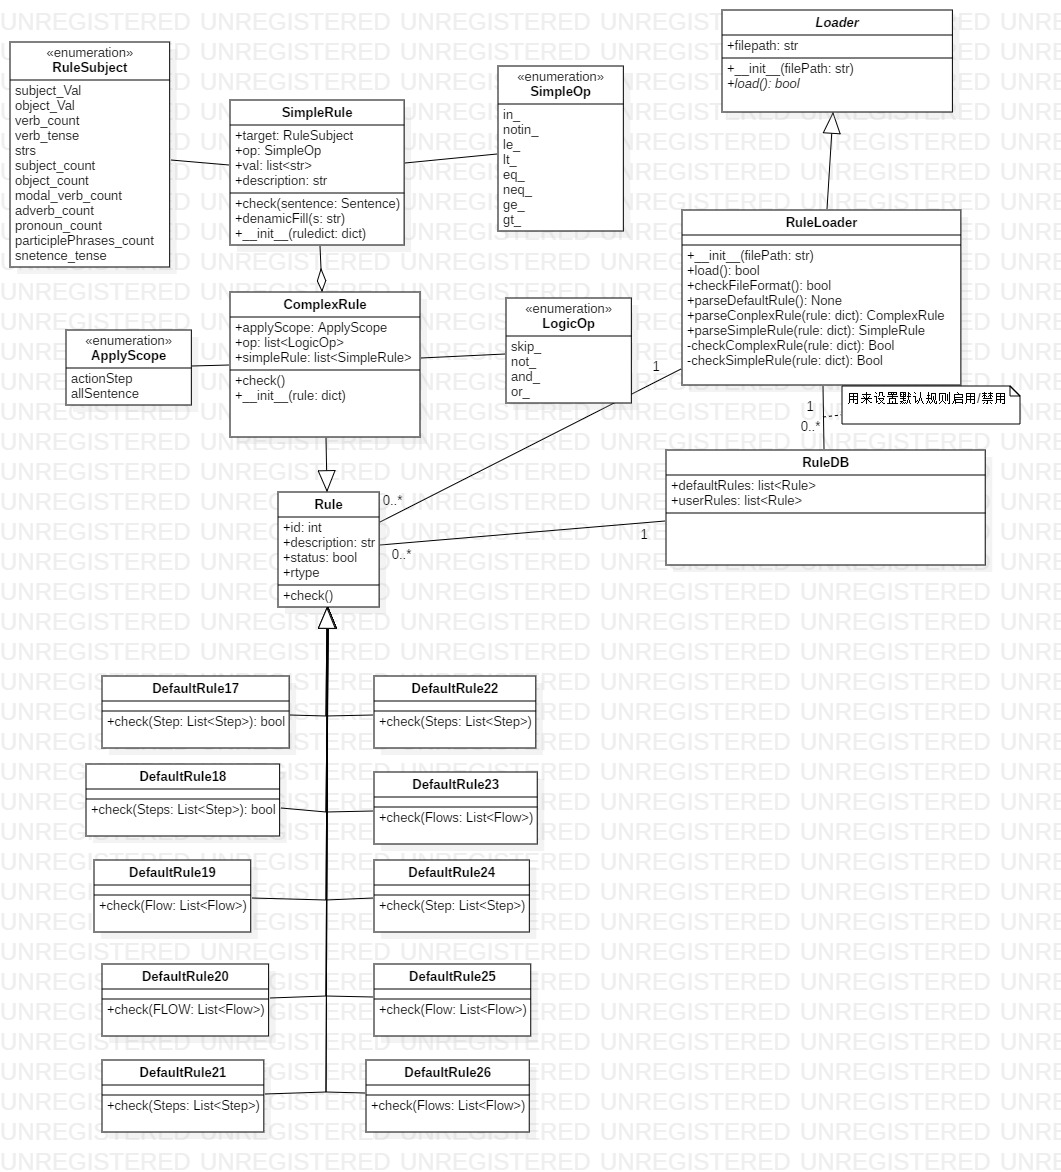
\includegraphics[width=1\textwidth]{./src/classDiagram_rule.jpg} 
    		\caption{规则解析与规则实体部分类图} 
    	\end{figure}
    \end{itemize}
	规则解析部分ocl:\\
	context: Loader\\
	inv: self.filepath <> None\\
	context:RucmLoader::load()\\
	postCondition: RUCMRooot.usecases.size() >0 and RUCMRooot.actors.size() >0\\ 
	context: RuleDB	\\
	inv: self.defaultRules <> None and self.userRules <> None\\
    \subsection{规则实体部分}
   	规则实体部分如图\ref{classDiagram_rule}所示。主要分为defaultRule,Rule,ComplexRule三大类。defaultRule实现关键字规则的检查,Rule是所有规则类的基类。ComplexRule负责所有形式化规则检查。
    \begin{itemize}

    
    \item	Rule:
    所有的规则都继承自rule基类,Rule的子类包括DefaultRuleXXX,ComplexRule(SimpleRule不是Rule的子类)。\\
    id:rule规则表示\\
    description:规则描述\\
    status:是否启用\\
    rtype:规则的类表,rtype必须取'user','system'之一
    \item	ComplexRule:\\
    一个复合规则可以由多个简单规则的检查结果综合而成\\
    applyScope:规则的作用域,目前作用于可以为rucm中的 action字段或者所有的句子。\\
    simpleRule:简单规则列表\\
    op:对简单规则的综合逻辑操作
    \item	SimpleRule:\\
    一个simpleRule只检查一个句子中的一个字段,它的检查方式可以抽象为某个句子成分在/不在目标列表中。\\
    target:要检查的句子成分,具体取值可以参见rule-template.md\\
    op:最检查目标的逻辑约束可以是in/not in\\
    val:允许/禁止列表\\
    check(setence:Sentence):检查句子\\
    dynamicFill:(s:str):动态填充val,比如填充rucm中的actor\\
    DefaultRuleXXX:\\
    无法被抽象成ComplexRule形式的规\\
\end{itemize}
    规则实体部分ocl:\\
    context: Rule\\
    inv: self.id >= 0 and self.description <> None and collection("user","system").includes(self.rtype)\\    
    context: ComplexRule\\
    inv: self.op <> None self.op.size() >0 and self.simpleRule.size() >0\\
    context: SimpleRule\\
    inv: self.val <> None and self.description <> None and self.val.size()>0 and 
    (if (collection(subject\_count,object\_count,verb\_count,modal\_verb\_count,adverb\_count,pronoun\_count).include(collection(self.subject))) then self.val.forAll(x|type(x) == Integer)else true)and
    (if collection(ge,gt,eq,neq,lt,le).include(self.op) then self.val.forAll(x|type(x) == Integer else true)\\
    context: SimpleRule::dynamicFill()\\
    postCondition:return=self.val.forAll(s:str|s.contain("\$") = Flase)
	
    \subsection{报告部分}
    \begin{itemize}
    	\item 	ErrorInfo:\\
    	包含检查错误结果的基本信息,包括检查出错误的规则,相应的用例名以及句子。
    	\item	Reporter:\\
    	静态类,用于生成报告。
    	\begin{figure}
    		\centering
    		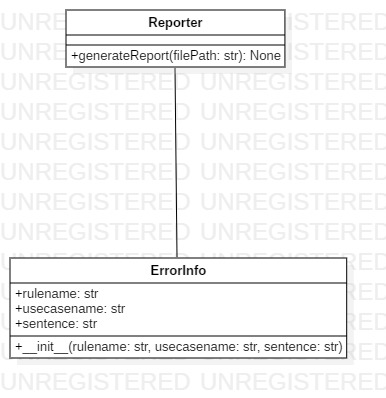
\includegraphics[width=.5\textwidth]{./src/classDiagram_report.jpg} 
    		\caption{报告部分类图} 
    	\end{figure}
    \end{itemize}
	
	报告部分ocl:\\
	context: ErrorInfo\\
	inv: self.rulename <> None and self.usecasename <> None and self.sentence <> None\\
	context:Reporter\\
	inv:self.errors <> None\\
	
    \subsection{RUCM部分}
  	我们为了方便规则类进行相应信息的获取,设置了RUCMRoot类对useceCase禁停统一管理,并且提供了对于sentence,Action等信息的痛惜查询接口。根据rucm文件结构与逻辑组织方式,我们从顶层到底层分别设置了Usecase,Flow,Action,Sentence,Word类。如此进行设置不仅方便RUCM的解析,也简化了后续的检查流程。
   	\begin{itemize}
   		\item 	RUCMRoot:\\
   		存储所有的RUCM信息包括actor列表域usecase列表,并且提供相应get方法方便rule查询信息\\
   		usecases:用例列表\\
   		actors:actor列表\\
   		getActors():获得actor列表\\
   		getAllSteps():获得所有step列表\\
   		getAllSentences():获得所有的句子\\
   		getUseCase(usecasename:str):查找相应的usecase
   		\item 	Usecase:\\
   		对应一个用例\\
   		id:用例id\\
   		name:usecase的名字\\
   		briefDescription:usecase简单描述\\
   		preConddition:前置条件\\
   		include:该用例所包含的用例\\
   		extend:该用例extend的用例\\
   		generalization:该用例泛化的用例\\
   		basicFlow:用例的基本流\\
   		specificFlows:用例分支流\\
   		findRfs(flowname:str,stepIndex:int)->bool:判断名字叫flowname的flow中是否存在序号stepIndex的步骤
   		\item 	Flow:\\
   		type:区分basicflow/Specific Flow/Global Alternative Flow\\
   		name:flow名称\\
   		postcondition:flow的postcondition\\
   		steps:构成flow的step\\
   		RfsStatement:specific flow的RFS字段\\
   		id:flow的id
   		\item 	step:\\
   		一个step可以由多个sentence构成\\
   		index:step的序号\\
   		val:step的字符串\\
   		sentences:step字句\\
   		parse\_step():解析句子
   		\item 	sentence:\\
   		一个sentence可以是一个正常的自然语言句子,也可以是一个关键字(IF/ELSE 等)\\
   		val:sentence字符串\\
   		nature:sentence的关键字类别
   		\item 	RUCMBase:\\
   		所有的RUCM元素的基类,提供向上查找父节点以及所属Usecase的相应属性
   		word:\\
   		val:词的字符串\\
   		type:词的类别(noun/adj/verb等)\\
   		tense:词的时态(past/present等)
   		\begin{figure}
   			\centering
   			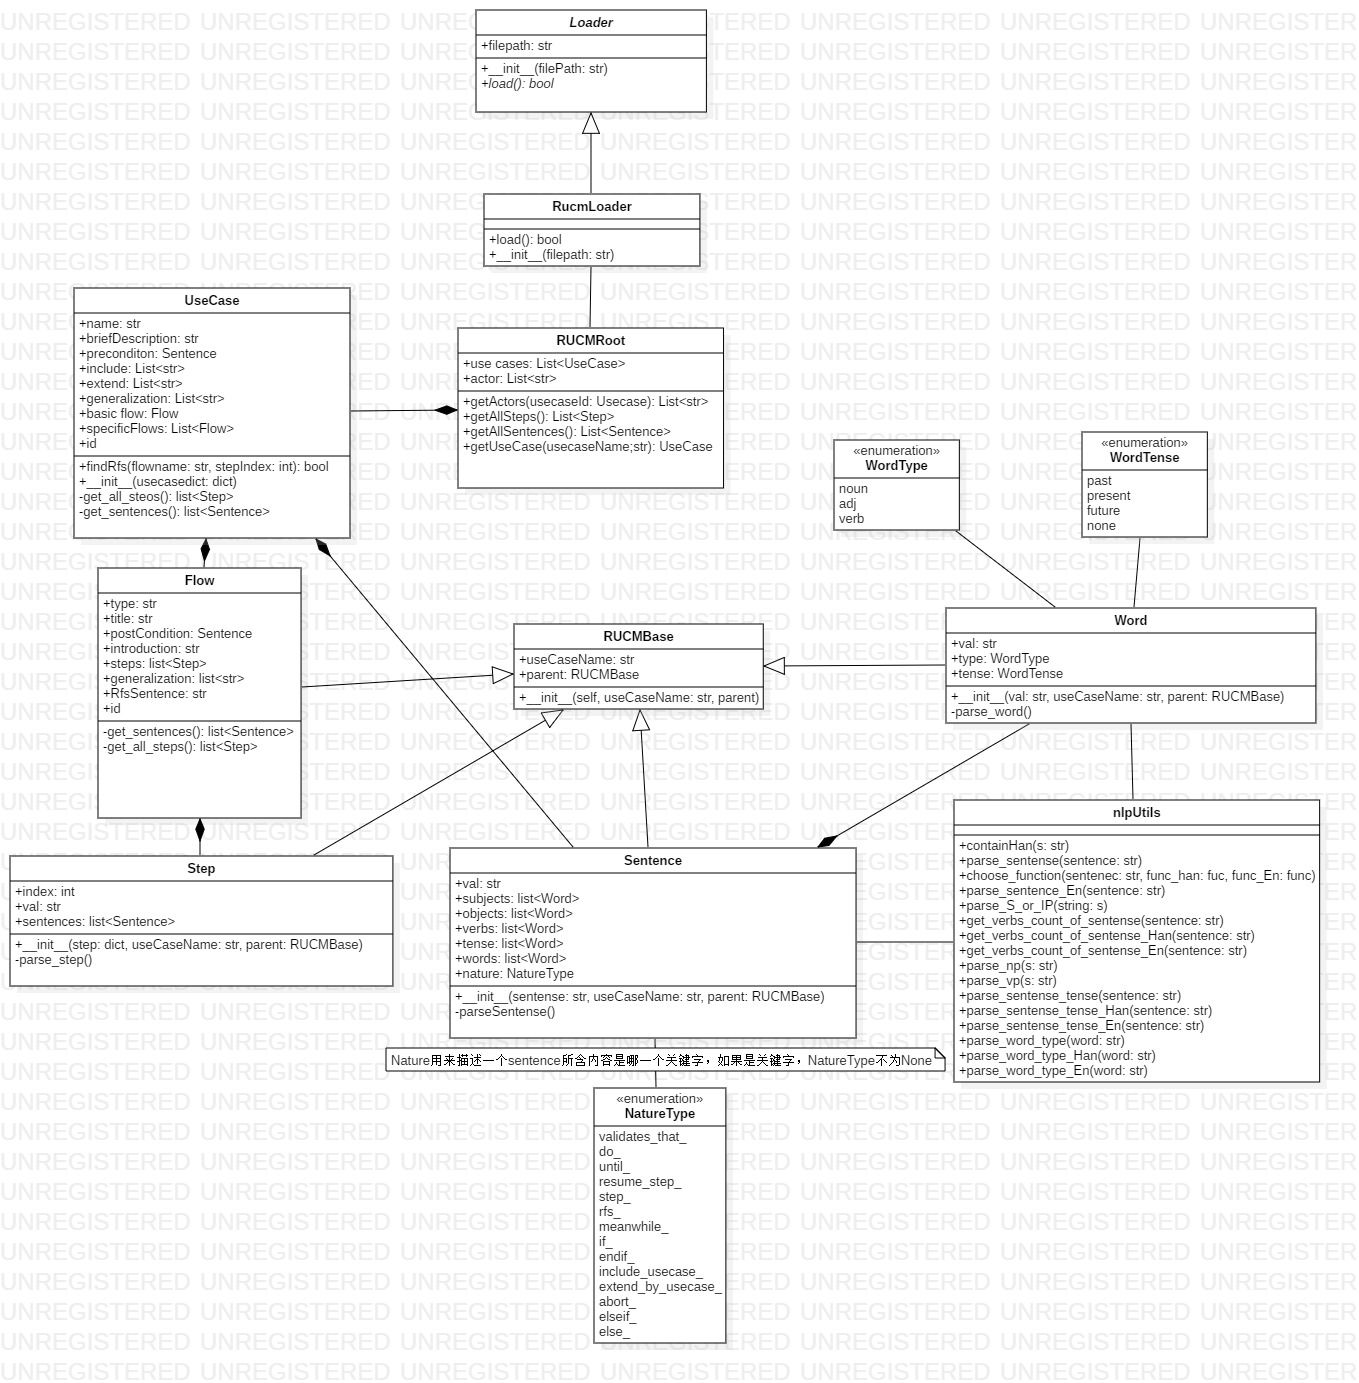
\includegraphics[width=1\textwidth]{./src/classDiagram_rucmElement.jpg} 
   			\caption{报告部分类图部分类图} 
   		\end{figure}
   	\end{itemize}
   	rucm部分ocl:\\
   	context:RucmLoader::load()\\
   	postCondition: RUCMRooot.usecases.size() >0 and RUCMRooot.actors.size() >0\\ 
   	context: Word\\
   	inv: self.val <> None and self.type <> None and self.tense <> None\\
   	context: Sentence\\
   	inv: self.val <> None and self.subjects <> None and self.objects <> None and self.verbs <> None and self.tense <> None and self.words <> None\\
   	context: Step\\
   	inv: self.index >= 0 and self.val <> None and self.sentences <> None and self.sentences.size() >0\\
   	context: Flow\\
   	inv: collection("BasicFlow","Specific Flow","Global Alternative Flow").includes(self.type) and self.title <> None and self.postCondition <> None and self.introduction <> None 	and self.steps <> None and self.steps.size() >0 and self.include <> None and self.extend <> None and self.generalization <> None and self.rfsSentence <> None\\
   	context: UseCase\\
   	inv: self.name <> None and self.briefDescription <> None and self.postCondition <> None and self.include <> None and self.extend <> None and self.generalization <> None	and self.basicFlow <> None and self.specificFlows <> None and self.id >= 0
   	
   
    \subsection{自然语言处理部分}
	如图\ref{classDiagram_nlputils}所示,该部分由多个方法组成,构成nulputils模块,该部分的主要功能是解析句子/词语成分,并且给予相应的自然语义标注。因为中文的语法分析与英文的语法分析有较大不同,我们设置XXX\_En和XXX\_Han对其进行分别处理。并且设置方法choose\_function对语言进行选择
    	\begin{figure}
	\centering
	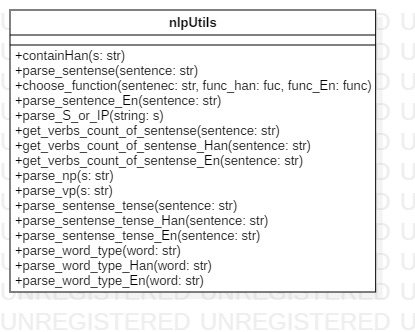
\includegraphics[width=.5\textwidth]{./src/classDiagram_nlputils.jpg} 
	\caption{自然语言处理部分类图} 
	\label{classDiagram_nlputils}
	\end{figure}
\begin{comment}
\section{用户规则设计}
rule文件有一个dict组成,其中有两个字段,分别是default 和user-def。分别代表默认规则列表和用户定义规则列表。\\
default字段下的数据尽量不要改,唯一可以改的是status字段,当status为false是,规则处于禁用状态\\
用户规则列表由用户规则聚合而成,一个用户规则下的字段包括:\\
\begin{itemize}
	
	\item 	id: 用户规则id,不能重复\\
	\item applyScope: 规则作用域,取值包括"actionStep"(flow中的句子),"allSentence"(RUCM中所有句子)
	\item simpleRules: 一个用户规则可以被看做多个简单规则的聚合,简单规则字典信息包括:
	\begin{itemize}
	\item subject: 规则要检查的对象,他的取值包括:
	\item subject\_Val: 主语的值
	\item subject\_count:主语的数量
	\item object\_Val: 宾语的值
	\item object\_count: 宾语的数量
	\item verb\_count : 动词的数量
	\item verb\_tense:动词的时态
	\item strs: 句子中所有的词
	\item	modal\_verb\_count:情态动词的数量
	\item	adverb\_count:副词的数量
	\item	pronoun\_count:代词的数量
	\end{itemize}
	\item	operation: 对检查对象的约束,可以是in/notin/le/lt/eq/neq/ge/gt,分别表示约束对象在/不在/小于等于/小于/等于/不等于/大于等于/小于
	\item	val: 约束列表,例如`{"subject":"subject\_Val", "operation": "in", "val":["system"]}`表示主语中不能出现system字眼。列表中除了出现正常字符串以外,还可以出现"\$actor"代表RUCM中的actor
	\item 注意:当subject字段为XX\_count的时候,val字段中只能出现数字,当operation为除了in notin以外的字段时候,val字段中只能出现数字。
	\item status:当status为false时,规则处于禁用状态
	\item	operation:综合简单规则的逻辑操作
	\item	第一个字符代表对整个检查结果的操作"-"代表无操作,"!"代表取非操作
	\item	第一个字符往后分别代表对于简单规则之间的逻辑操作,"\&"代表与操作,“|”代表或操作
	\item	description:规则描述
	\item	注意:通过规则模板编辑方式可以编写内含多个条件约束的规则,而通过GUI编辑方式获得的规则只能包含一个条件约束。
\end{itemize}
\end{comment}
\section{运行流程说明}
\subsection{rucm解析流程}
   	\begin{figure}
	\centering
	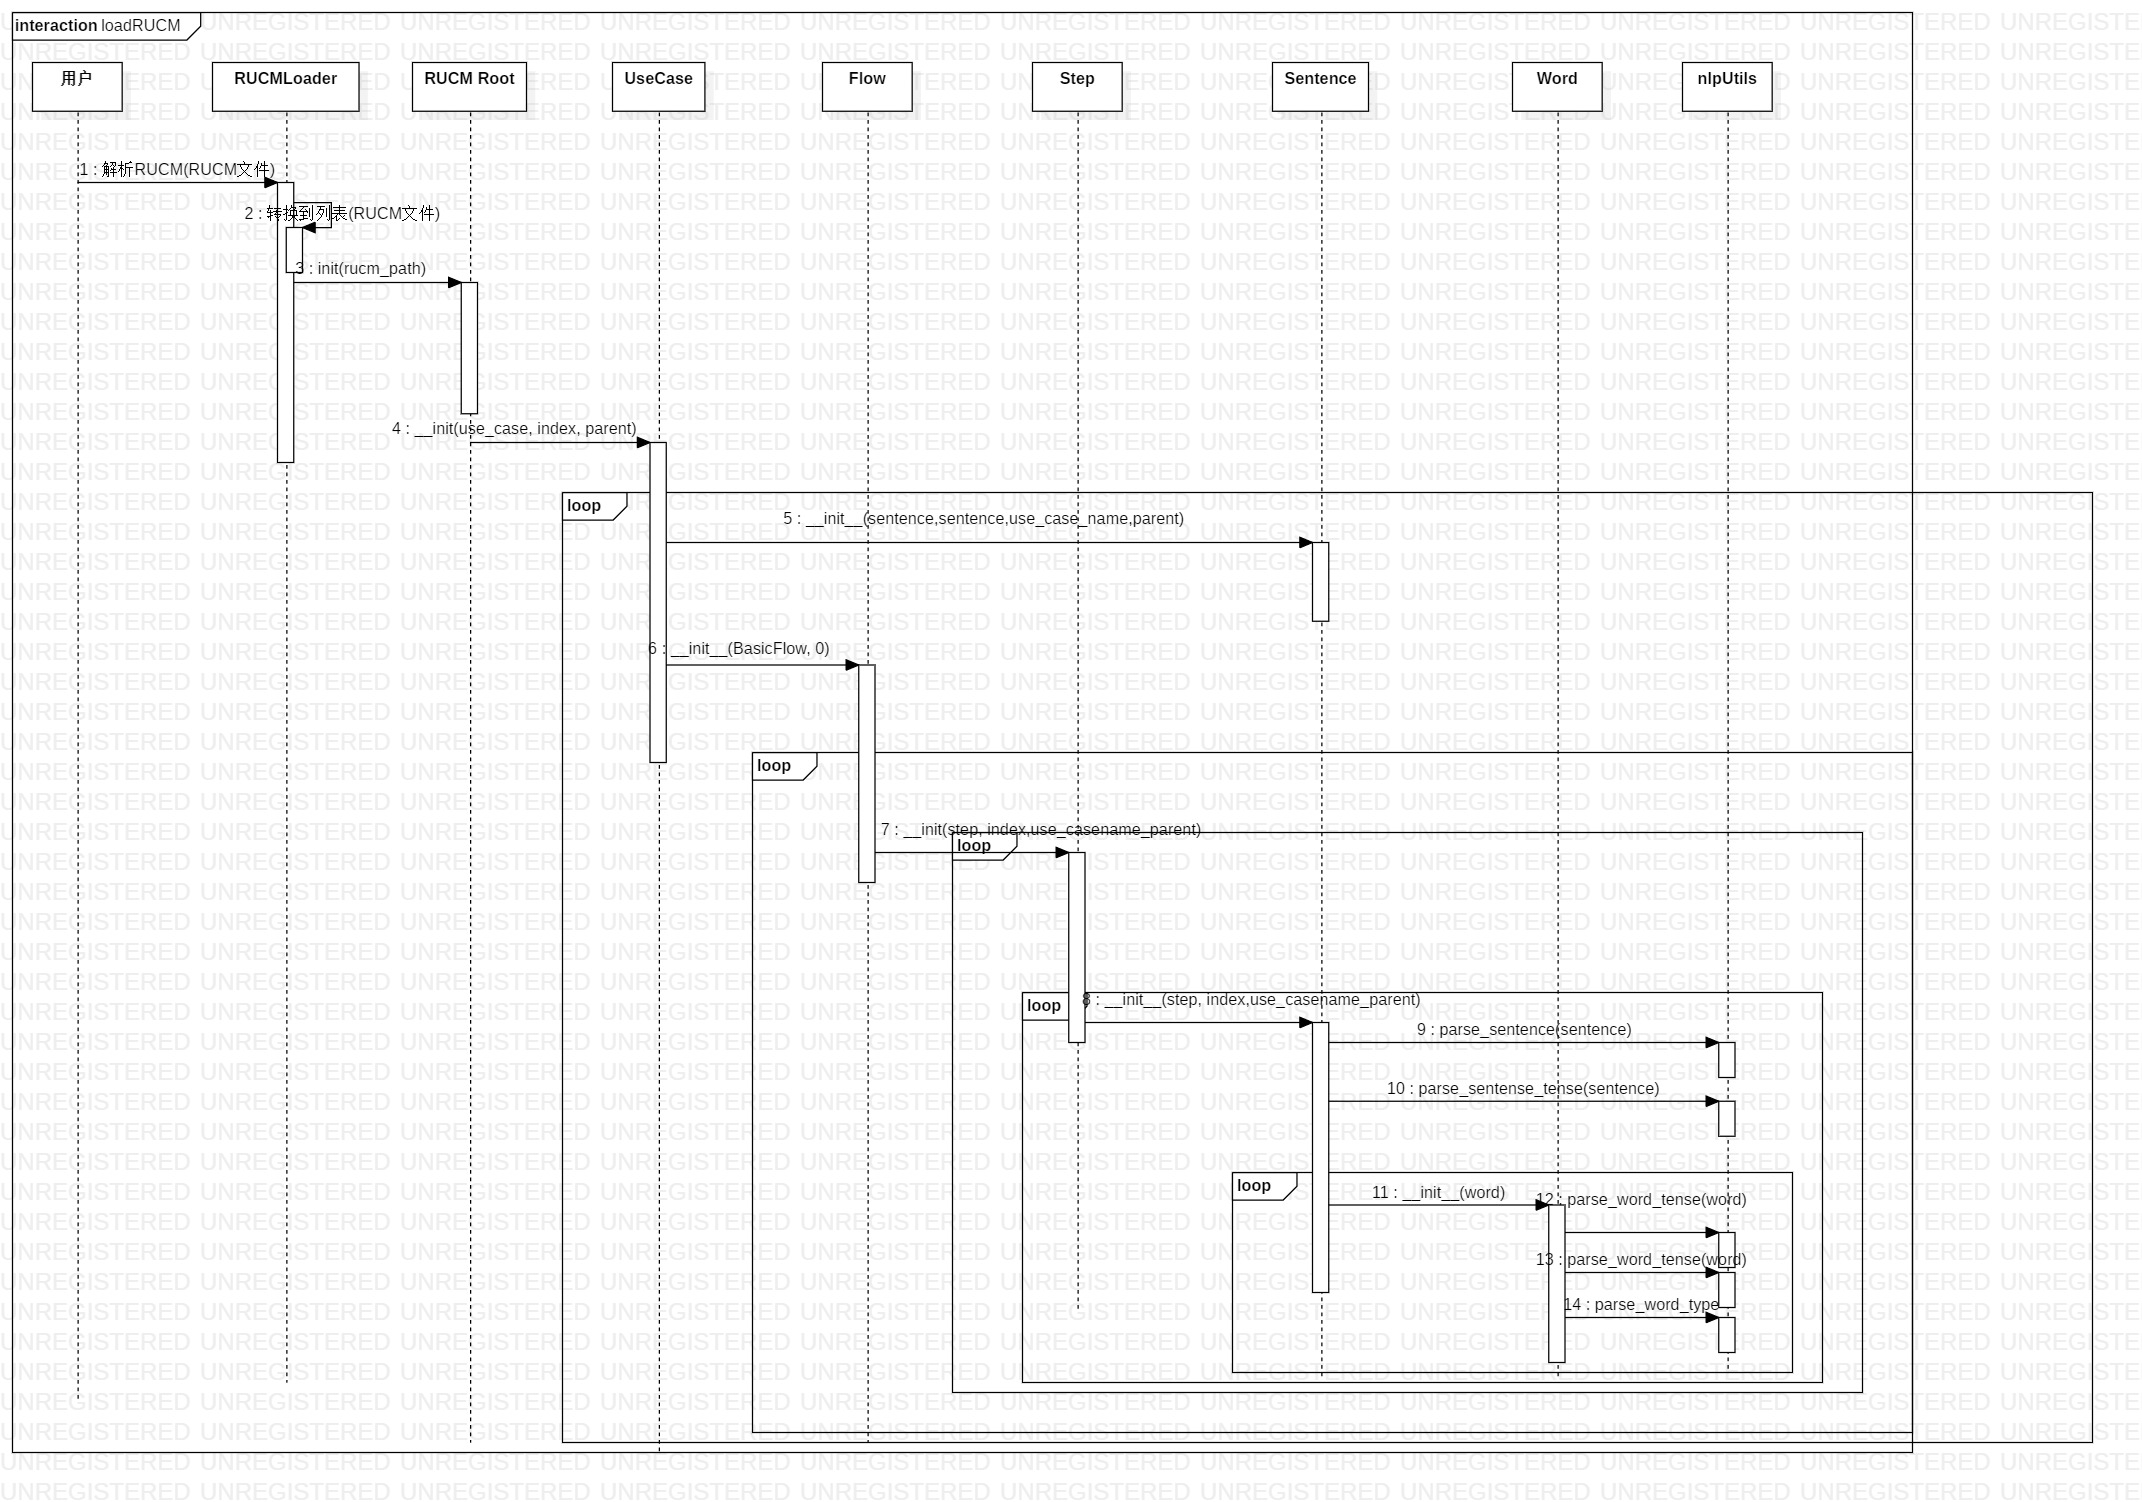
\includegraphics[width=1\textwidth]{./src/sequence_loadRUCM.jpg} 
	\caption{rucm解析流程图} 
	\label{sequence_loadRUCM}
	\end{figure}
	rucm解析流程如图\ref{sequence_loadRUCM}所示,rucmLoader通过调用RUCMRoot的init方法生成rucm相关类的实例。具体来说,rucm的解析是useCase,Flow,Step,Sentence,word等类依次反复迭代调用的过程。在生成Sentence和Word的过程中,sentence和word会调用自然语言处理模块获得相应的语法标注。

\subsection{规则解析流程}
   	\begin{figure}
	\centering
	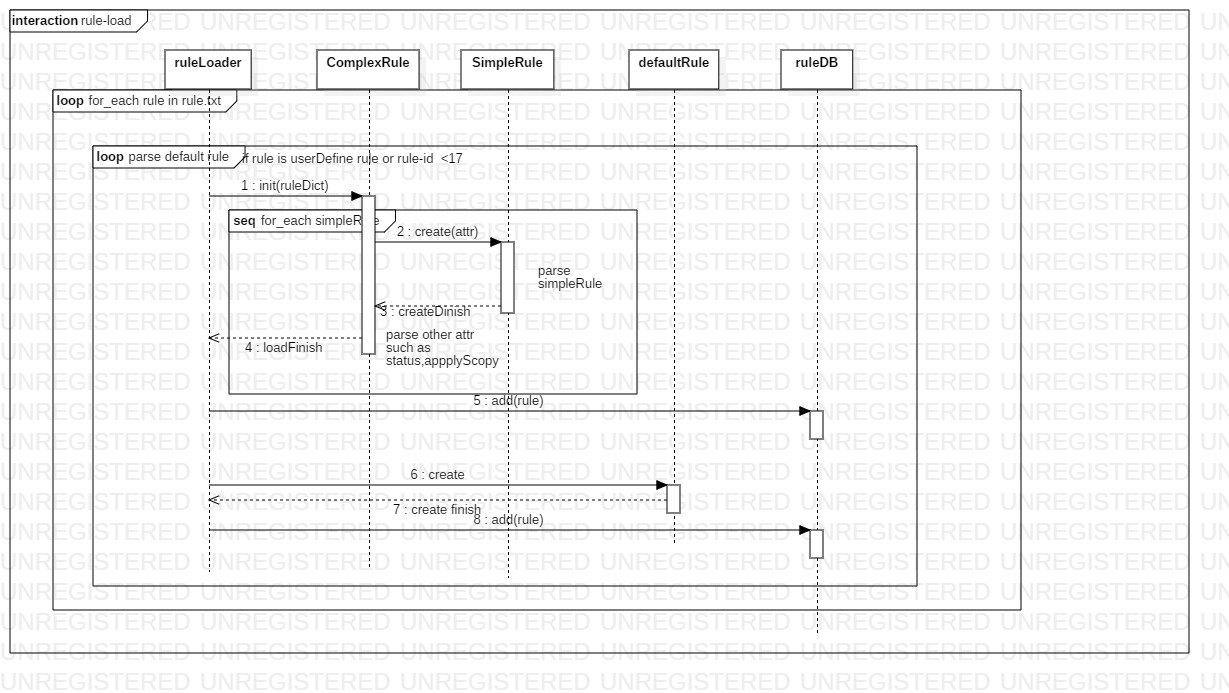
\includegraphics[width=1\textwidth]{./src/sequence_ruleLoad.jpg} 
	\caption{规则装载流程}
	\label{sequence_ruleLoad}
\end{figure}
	规则解析流程如图\ref{sequence_ruleLoad}所示规则解析分为两个部分,默认关键字规则解析和复杂规则解析,默认规则解析就是把对应id的规则实例化。而复杂规则的解析分为解析相应的简单子规则和解析复杂规则相应字段连个部分。当规则解析完毕后,规则被添加到了规则数据库中。
\subsection{复杂规则检查流程}
	\begin{figure}
	\centering
	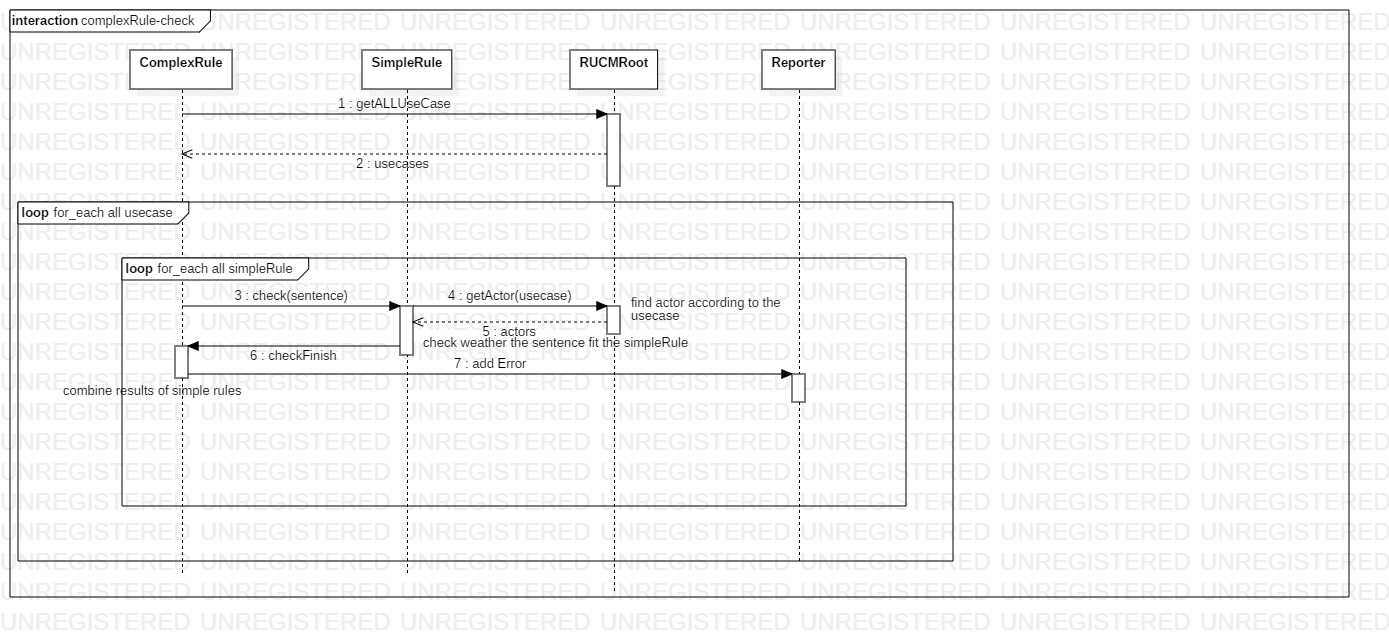
\includegraphics[width=1\textwidth]{./src/sequence_complexCheck.jpg} 
	\caption{rucm解析流程图} 
	\label{sequence_complexCheck}
	\end{figure}
	复杂规则解析流程如图\ref{sequence_complexCheck}所示。一个复杂规则可以由多个简单规则的检查结果综合而成。在进行复杂规则检查的时候,复杂规则先对下属的简单规则进行检查,待检查完成的时候将简单规则的检查见过进行综合获得最终检查结果。因为有些规则的约束值因rucm的文件不同而不同(如对actor的约束就是因rucm文件变化而变化的)

\subsection{gui状态转移说明}
	\begin{figure}
	\centering
	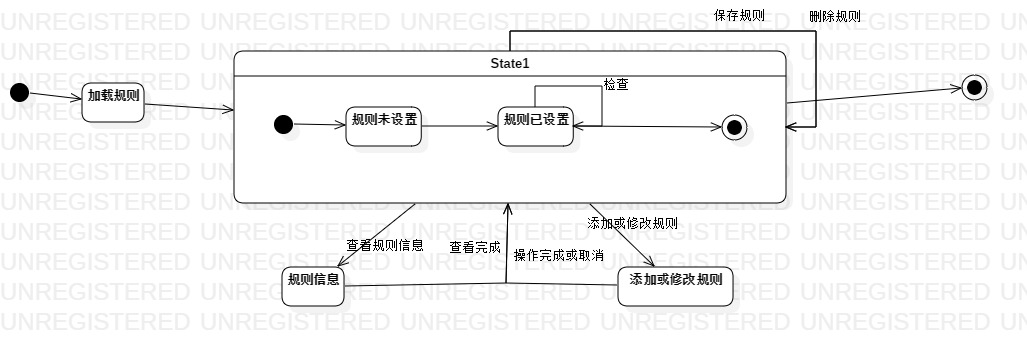
\includegraphics[width=1\textwidth]{./src/stateDisgram_gui.jpg} 
	\caption{图形界面状态转移图} 
	\label{stateDisgram_gui}
	\end{figure}
	gui状态转移如图\ref{stateDisgram_gui}所示。图形界面主要状态有三个:加载规则状态,就绪-rucm文件未设置状态和就绪rucm文件设置完成状态。两个就绪状态分别可以迁移到查看规则和添加/修改规则状态。通过设置rucm文件可以将"就绪-rucm文件未设置"状态迁移到“就绪-rucm文件设置完成”状态。当检查完成后,状态机返回“就绪-rucm文件未设置”状态
	
	
	
	